% Options for packages loaded elsewhere
\PassOptionsToPackage{unicode}{hyperref}
\PassOptionsToPackage{hyphens}{url}
\PassOptionsToPackage{dvipsnames,svgnames,x11names}{xcolor}
%
\documentclass[
  letterpaper,
  DIV=11,
  numbers=noendperiod]{scrartcl}

\usepackage{amsmath,amssymb}
\usepackage{iftex}
\ifPDFTeX
  \usepackage[T1]{fontenc}
  \usepackage[utf8]{inputenc}
  \usepackage{textcomp} % provide euro and other symbols
\else % if luatex or xetex
  \usepackage{unicode-math}
  \defaultfontfeatures{Scale=MatchLowercase}
  \defaultfontfeatures[\rmfamily]{Ligatures=TeX,Scale=1}
\fi
\usepackage{lmodern}
\ifPDFTeX\else  
    % xetex/luatex font selection
\fi
% Use upquote if available, for straight quotes in verbatim environments
\IfFileExists{upquote.sty}{\usepackage{upquote}}{}
\IfFileExists{microtype.sty}{% use microtype if available
  \usepackage[]{microtype}
  \UseMicrotypeSet[protrusion]{basicmath} % disable protrusion for tt fonts
}{}
\makeatletter
\@ifundefined{KOMAClassName}{% if non-KOMA class
  \IfFileExists{parskip.sty}{%
    \usepackage{parskip}
  }{% else
    \setlength{\parindent}{0pt}
    \setlength{\parskip}{6pt plus 2pt minus 1pt}}
}{% if KOMA class
  \KOMAoptions{parskip=half}}
\makeatother
\usepackage{xcolor}
\setlength{\emergencystretch}{3em} % prevent overfull lines
\setcounter{secnumdepth}{-\maxdimen} % remove section numbering
% Make \paragraph and \subparagraph free-standing
\ifx\paragraph\undefined\else
  \let\oldparagraph\paragraph
  \renewcommand{\paragraph}[1]{\oldparagraph{#1}\mbox{}}
\fi
\ifx\subparagraph\undefined\else
  \let\oldsubparagraph\subparagraph
  \renewcommand{\subparagraph}[1]{\oldsubparagraph{#1}\mbox{}}
\fi

\usepackage{color}
\usepackage{fancyvrb}
\newcommand{\VerbBar}{|}
\newcommand{\VERB}{\Verb[commandchars=\\\{\}]}
\DefineVerbatimEnvironment{Highlighting}{Verbatim}{commandchars=\\\{\}}
% Add ',fontsize=\small' for more characters per line
\usepackage{framed}
\definecolor{shadecolor}{RGB}{241,243,245}
\newenvironment{Shaded}{\begin{snugshade}}{\end{snugshade}}
\newcommand{\AlertTok}[1]{\textcolor[rgb]{0.68,0.00,0.00}{#1}}
\newcommand{\AnnotationTok}[1]{\textcolor[rgb]{0.37,0.37,0.37}{#1}}
\newcommand{\AttributeTok}[1]{\textcolor[rgb]{0.40,0.45,0.13}{#1}}
\newcommand{\BaseNTok}[1]{\textcolor[rgb]{0.68,0.00,0.00}{#1}}
\newcommand{\BuiltInTok}[1]{\textcolor[rgb]{0.00,0.23,0.31}{#1}}
\newcommand{\CharTok}[1]{\textcolor[rgb]{0.13,0.47,0.30}{#1}}
\newcommand{\CommentTok}[1]{\textcolor[rgb]{0.37,0.37,0.37}{#1}}
\newcommand{\CommentVarTok}[1]{\textcolor[rgb]{0.37,0.37,0.37}{\textit{#1}}}
\newcommand{\ConstantTok}[1]{\textcolor[rgb]{0.56,0.35,0.01}{#1}}
\newcommand{\ControlFlowTok}[1]{\textcolor[rgb]{0.00,0.23,0.31}{#1}}
\newcommand{\DataTypeTok}[1]{\textcolor[rgb]{0.68,0.00,0.00}{#1}}
\newcommand{\DecValTok}[1]{\textcolor[rgb]{0.68,0.00,0.00}{#1}}
\newcommand{\DocumentationTok}[1]{\textcolor[rgb]{0.37,0.37,0.37}{\textit{#1}}}
\newcommand{\ErrorTok}[1]{\textcolor[rgb]{0.68,0.00,0.00}{#1}}
\newcommand{\ExtensionTok}[1]{\textcolor[rgb]{0.00,0.23,0.31}{#1}}
\newcommand{\FloatTok}[1]{\textcolor[rgb]{0.68,0.00,0.00}{#1}}
\newcommand{\FunctionTok}[1]{\textcolor[rgb]{0.28,0.35,0.67}{#1}}
\newcommand{\ImportTok}[1]{\textcolor[rgb]{0.00,0.46,0.62}{#1}}
\newcommand{\InformationTok}[1]{\textcolor[rgb]{0.37,0.37,0.37}{#1}}
\newcommand{\KeywordTok}[1]{\textcolor[rgb]{0.00,0.23,0.31}{#1}}
\newcommand{\NormalTok}[1]{\textcolor[rgb]{0.00,0.23,0.31}{#1}}
\newcommand{\OperatorTok}[1]{\textcolor[rgb]{0.37,0.37,0.37}{#1}}
\newcommand{\OtherTok}[1]{\textcolor[rgb]{0.00,0.23,0.31}{#1}}
\newcommand{\PreprocessorTok}[1]{\textcolor[rgb]{0.68,0.00,0.00}{#1}}
\newcommand{\RegionMarkerTok}[1]{\textcolor[rgb]{0.00,0.23,0.31}{#1}}
\newcommand{\SpecialCharTok}[1]{\textcolor[rgb]{0.37,0.37,0.37}{#1}}
\newcommand{\SpecialStringTok}[1]{\textcolor[rgb]{0.13,0.47,0.30}{#1}}
\newcommand{\StringTok}[1]{\textcolor[rgb]{0.13,0.47,0.30}{#1}}
\newcommand{\VariableTok}[1]{\textcolor[rgb]{0.07,0.07,0.07}{#1}}
\newcommand{\VerbatimStringTok}[1]{\textcolor[rgb]{0.13,0.47,0.30}{#1}}
\newcommand{\WarningTok}[1]{\textcolor[rgb]{0.37,0.37,0.37}{\textit{#1}}}

\providecommand{\tightlist}{%
  \setlength{\itemsep}{0pt}\setlength{\parskip}{0pt}}\usepackage{longtable,booktabs,array}
\usepackage{calc} % for calculating minipage widths
% Correct order of tables after \paragraph or \subparagraph
\usepackage{etoolbox}
\makeatletter
\patchcmd\longtable{\par}{\if@noskipsec\mbox{}\fi\par}{}{}
\makeatother
% Allow footnotes in longtable head/foot
\IfFileExists{footnotehyper.sty}{\usepackage{footnotehyper}}{\usepackage{footnote}}
\makesavenoteenv{longtable}
\usepackage{graphicx}
\makeatletter
\def\maxwidth{\ifdim\Gin@nat@width>\linewidth\linewidth\else\Gin@nat@width\fi}
\def\maxheight{\ifdim\Gin@nat@height>\textheight\textheight\else\Gin@nat@height\fi}
\makeatother
% Scale images if necessary, so that they will not overflow the page
% margins by default, and it is still possible to overwrite the defaults
% using explicit options in \includegraphics[width, height, ...]{}
\setkeys{Gin}{width=\maxwidth,height=\maxheight,keepaspectratio}
% Set default figure placement to htbp
\makeatletter
\def\fps@figure{htbp}
\makeatother

\KOMAoption{captions}{tableheading}
\makeatletter
\makeatother
\makeatletter
\makeatother
\makeatletter
\@ifpackageloaded{caption}{}{\usepackage{caption}}
\AtBeginDocument{%
\ifdefined\contentsname
  \renewcommand*\contentsname{Table of contents}
\else
  \newcommand\contentsname{Table of contents}
\fi
\ifdefined\listfigurename
  \renewcommand*\listfigurename{List of Figures}
\else
  \newcommand\listfigurename{List of Figures}
\fi
\ifdefined\listtablename
  \renewcommand*\listtablename{List of Tables}
\else
  \newcommand\listtablename{List of Tables}
\fi
\ifdefined\figurename
  \renewcommand*\figurename{Figure}
\else
  \newcommand\figurename{Figure}
\fi
\ifdefined\tablename
  \renewcommand*\tablename{Table}
\else
  \newcommand\tablename{Table}
\fi
}
\@ifpackageloaded{float}{}{\usepackage{float}}
\floatstyle{ruled}
\@ifundefined{c@chapter}{\newfloat{codelisting}{h}{lop}}{\newfloat{codelisting}{h}{lop}[chapter]}
\floatname{codelisting}{Listing}
\newcommand*\listoflistings{\listof{codelisting}{List of Listings}}
\makeatother
\makeatletter
\@ifpackageloaded{caption}{}{\usepackage{caption}}
\@ifpackageloaded{subcaption}{}{\usepackage{subcaption}}
\makeatother
\makeatletter
\@ifpackageloaded{tcolorbox}{}{\usepackage[skins,breakable]{tcolorbox}}
\makeatother
\makeatletter
\@ifundefined{shadecolor}{\definecolor{shadecolor}{rgb}{.97, .97, .97}}
\makeatother
\makeatletter
\makeatother
\makeatletter
\makeatother
\ifLuaTeX
  \usepackage{selnolig}  % disable illegal ligatures
\fi
\IfFileExists{bookmark.sty}{\usepackage{bookmark}}{\usepackage{hyperref}}
\IfFileExists{xurl.sty}{\usepackage{xurl}}{} % add URL line breaks if available
\urlstyle{same} % disable monospaced font for URLs
\hypersetup{
  pdftitle={Case study: Spanish Flu in London, Birmingham, and Liverpool},
  pdfauthor={Qianying (Ruby) Lin; Spencer J. Fox; Zian (Larry) Zhuang},
  colorlinks=true,
  linkcolor={blue},
  filecolor={Maroon},
  citecolor={Blue},
  urlcolor={Blue},
  pdfcreator={LaTeX via pandoc}}

\title{Case study: Spanish Flu in London, Birmingham, and Liverpool}
\author{Qianying (Ruby) Lin \and Spencer J. Fox \and Zian (Larry)
Zhuang}
\date{}

\begin{document}
\maketitle
\ifdefined\Shaded\renewenvironment{Shaded}{\begin{tcolorbox}[interior hidden, breakable, sharp corners, boxrule=0pt, borderline west={3pt}{0pt}{shadecolor}, frame hidden, enhanced]}{\end{tcolorbox}}\fi

\hypertarget{objectives}{%
\subsection{Objectives}\label{objectives}}

\begin{enumerate}
\def\labelenumi{\arabic{enumi}.}
\tightlist
\item
  To explore the use of POMP models in the context of meta-populations
  and multiple waves.
\item
  To illustrate the use of POMP models in a more complex setting.
\item
  To demonstrate the use of diagnostic probes for model criticism.
\item
  To provide an example that can be modified to apply similar approaches
  to other outbreaks of emerging infectious diseases.
\end{enumerate}

\vspace{2ex}

\hypertarget{spanish-flu-pandemic}{%
\section{1918 Spanish Flu Pandemic}\label{spanish-flu-pandemic}}

\hypertarget{emerging-infectious-disease-pandemic}{%
\subsection{Emerging infectious disease
pandemic}\label{emerging-infectious-disease-pandemic}}

\begin{itemize}
\tightlist
\item
  The 1918 Spanish flu pandemic was one of the deadliest pandemics in
  human history.
\item
  The pandemic lasted from January 1918 to December 1920, spreading to
  nearly every part of the world.
\item
  The pandemic was caused by the H1N1 influenza A virus.
\item
  The pandemic was responsible for the deaths of an estimated 50 million
  people worldwide.
\end{itemize}

\framebreak

Key questions included:

\begin{enumerate}
\def\labelenumi{\arabic{enumi}.}
\tightlist
\item
  How fast will the pandemic unfold?
\item
  What are the common and differentiated characteristics of the pandemic
  in different cities?
\item
  How people will correspond to the pandemic?
\end{enumerate}

\hypertarget{data-and-model}{%
\section{Data and model}\label{data-and-model}}

\hypertarget{weekly-reported-data}{%
\subsection{Weekly reported data}\label{weekly-reported-data}}

\begin{Shaded}
\begin{Highlighting}[]
\NormalTok{dat }\OtherTok{\textless{}{-}} \FunctionTok{read\_csv}\NormalTok{(}\StringTok{"1918flu\_3cities\_1wave.csv"}\NormalTok{)}
\FunctionTok{head}\NormalTok{(dat)}
\end{Highlighting}
\end{Shaded}

\begin{verbatim}
# A tibble: 6 x 5
  London Birmingham Liverpool  week date      
   <dbl>      <dbl>     <dbl> <dbl> <date>    
1     13          2         2     1 1918-09-21
2     17          1        16     2 1918-09-28
3     25          2        34     3 1918-10-05
4    110          3       127     4 1918-10-12
5    519         15       226     5 1918-10-19
6   1579         60       211     6 1918-10-26
\end{verbatim}

\framebreak

\begin{figure}[h!]

{\centering 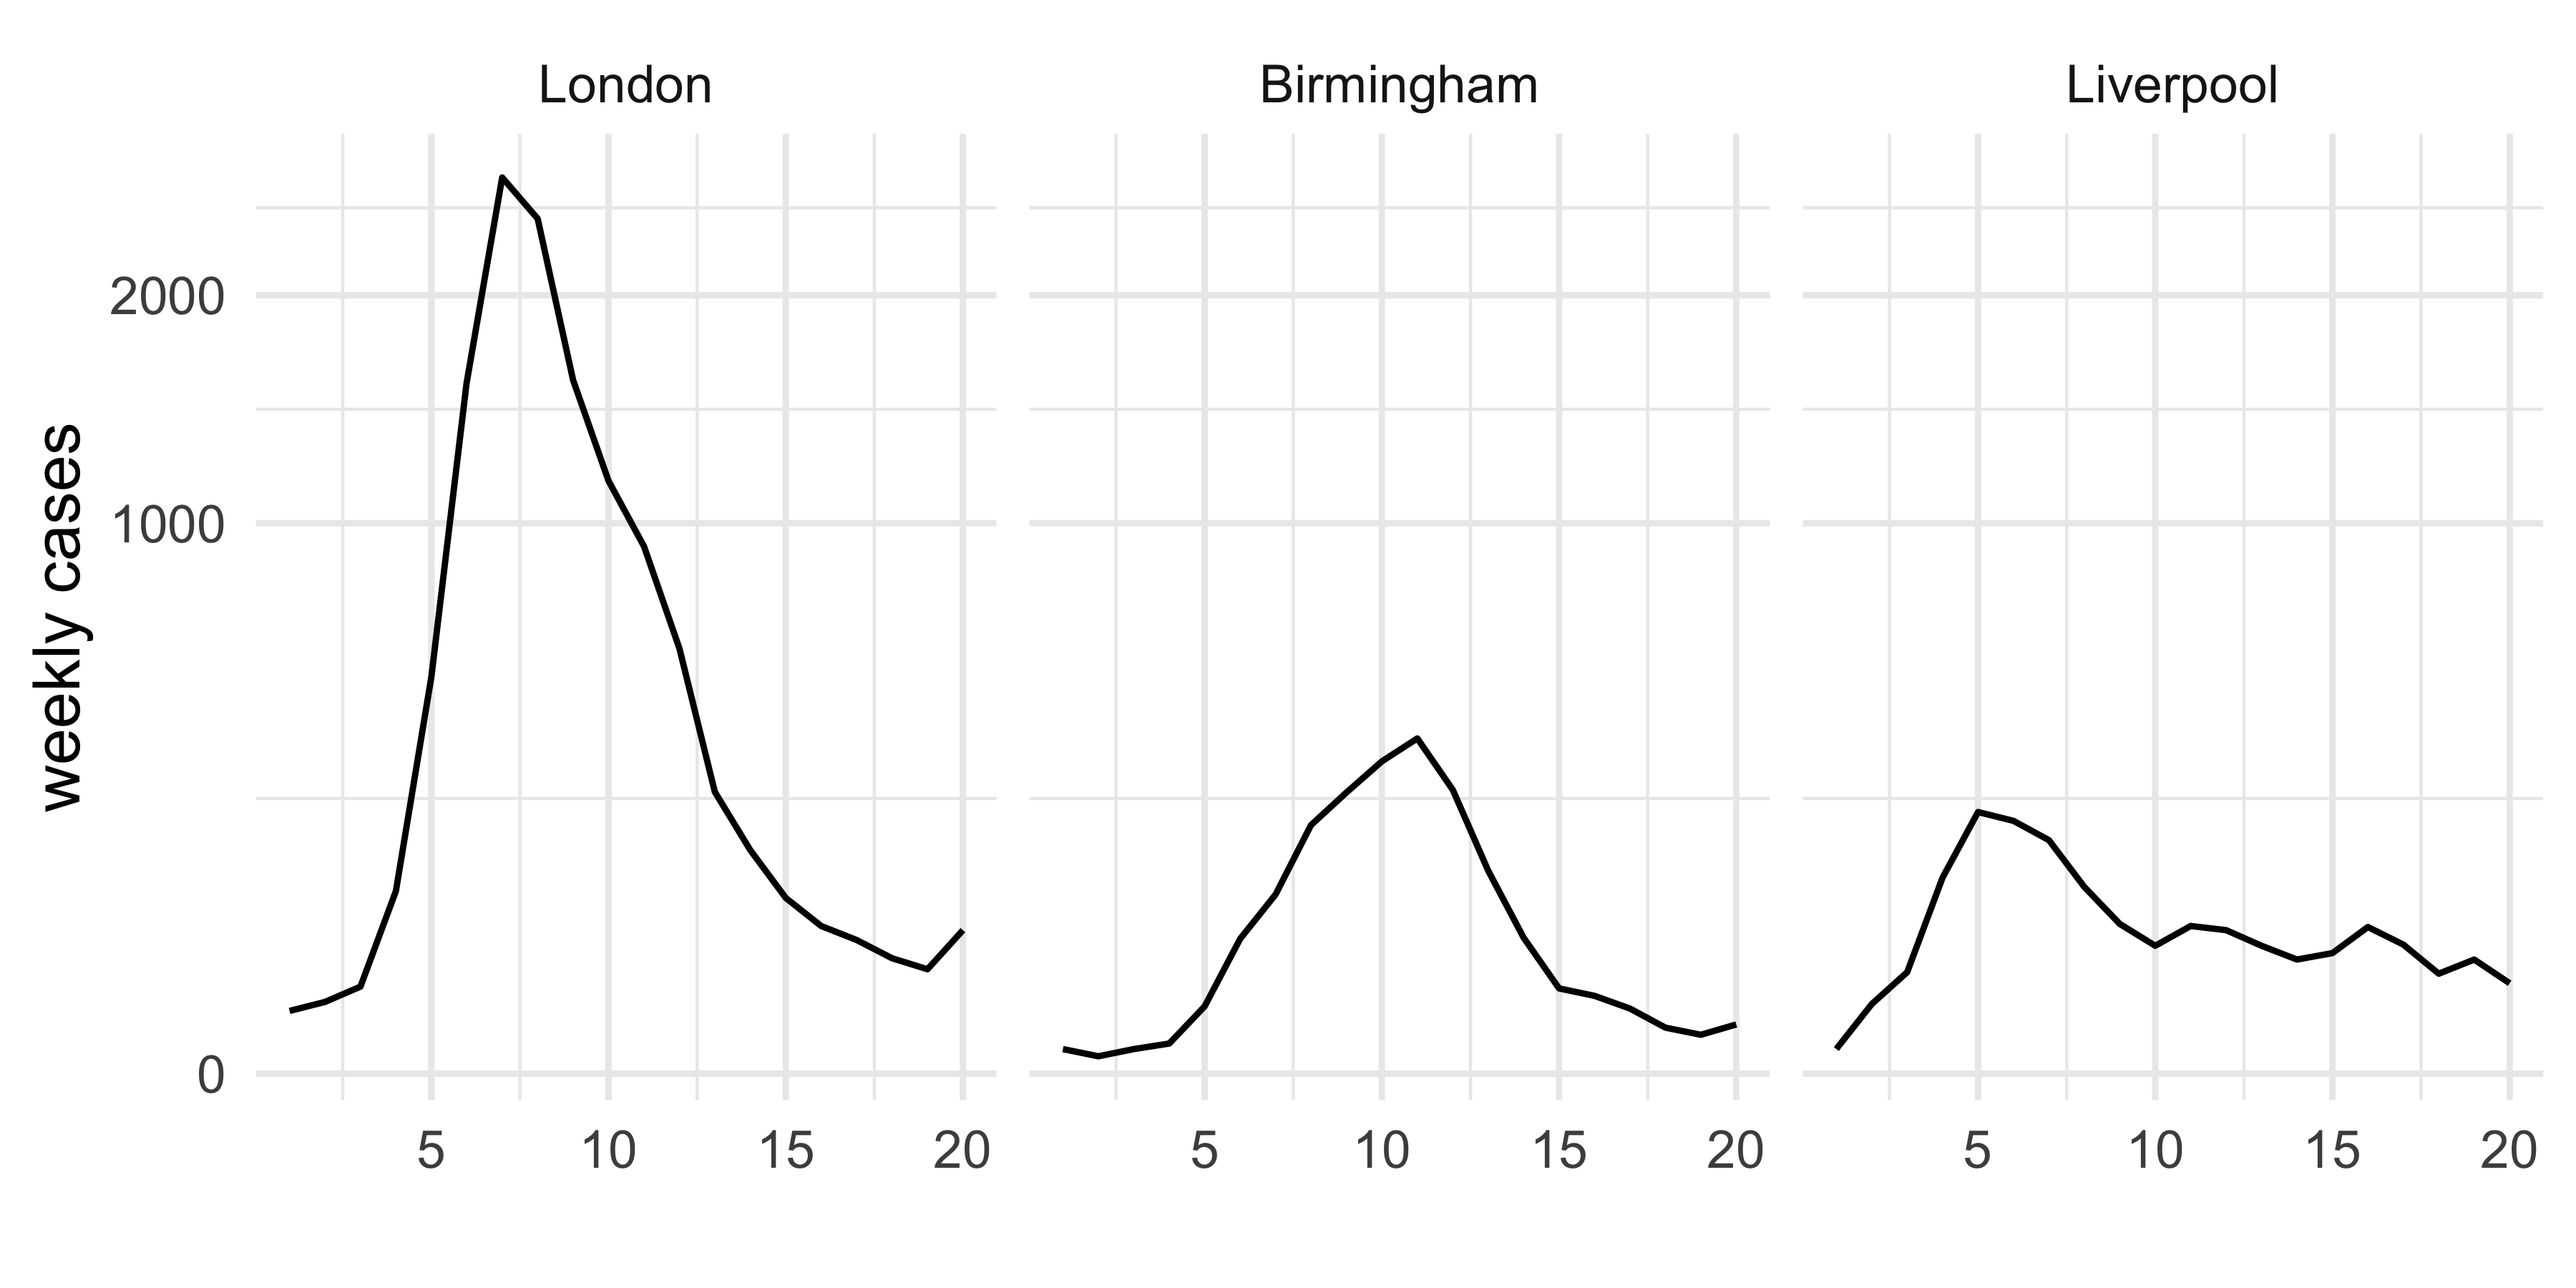
\includegraphics[width=\textwidth,height=0.9\textheight]{tmp//figure/plot-1.png}

}

\end{figure}

\hypertarget{sir-model-with-behavioral-response}{%
\subsection{SIR model with behavioral
response}\label{sir-model-with-behavioral-response}}

\begin{itemize}
\tightlist
\item
  Social distancing is a common public health intervention.
\item
  We model the effect of social distancing as a reduction in the
  transmission rate.
\item
  We incorporate demographic and climatic features to model the spread
  of the disease.
\item
  The SIR model with behavioral response is given by:
\end{itemize}

\begin{center}
    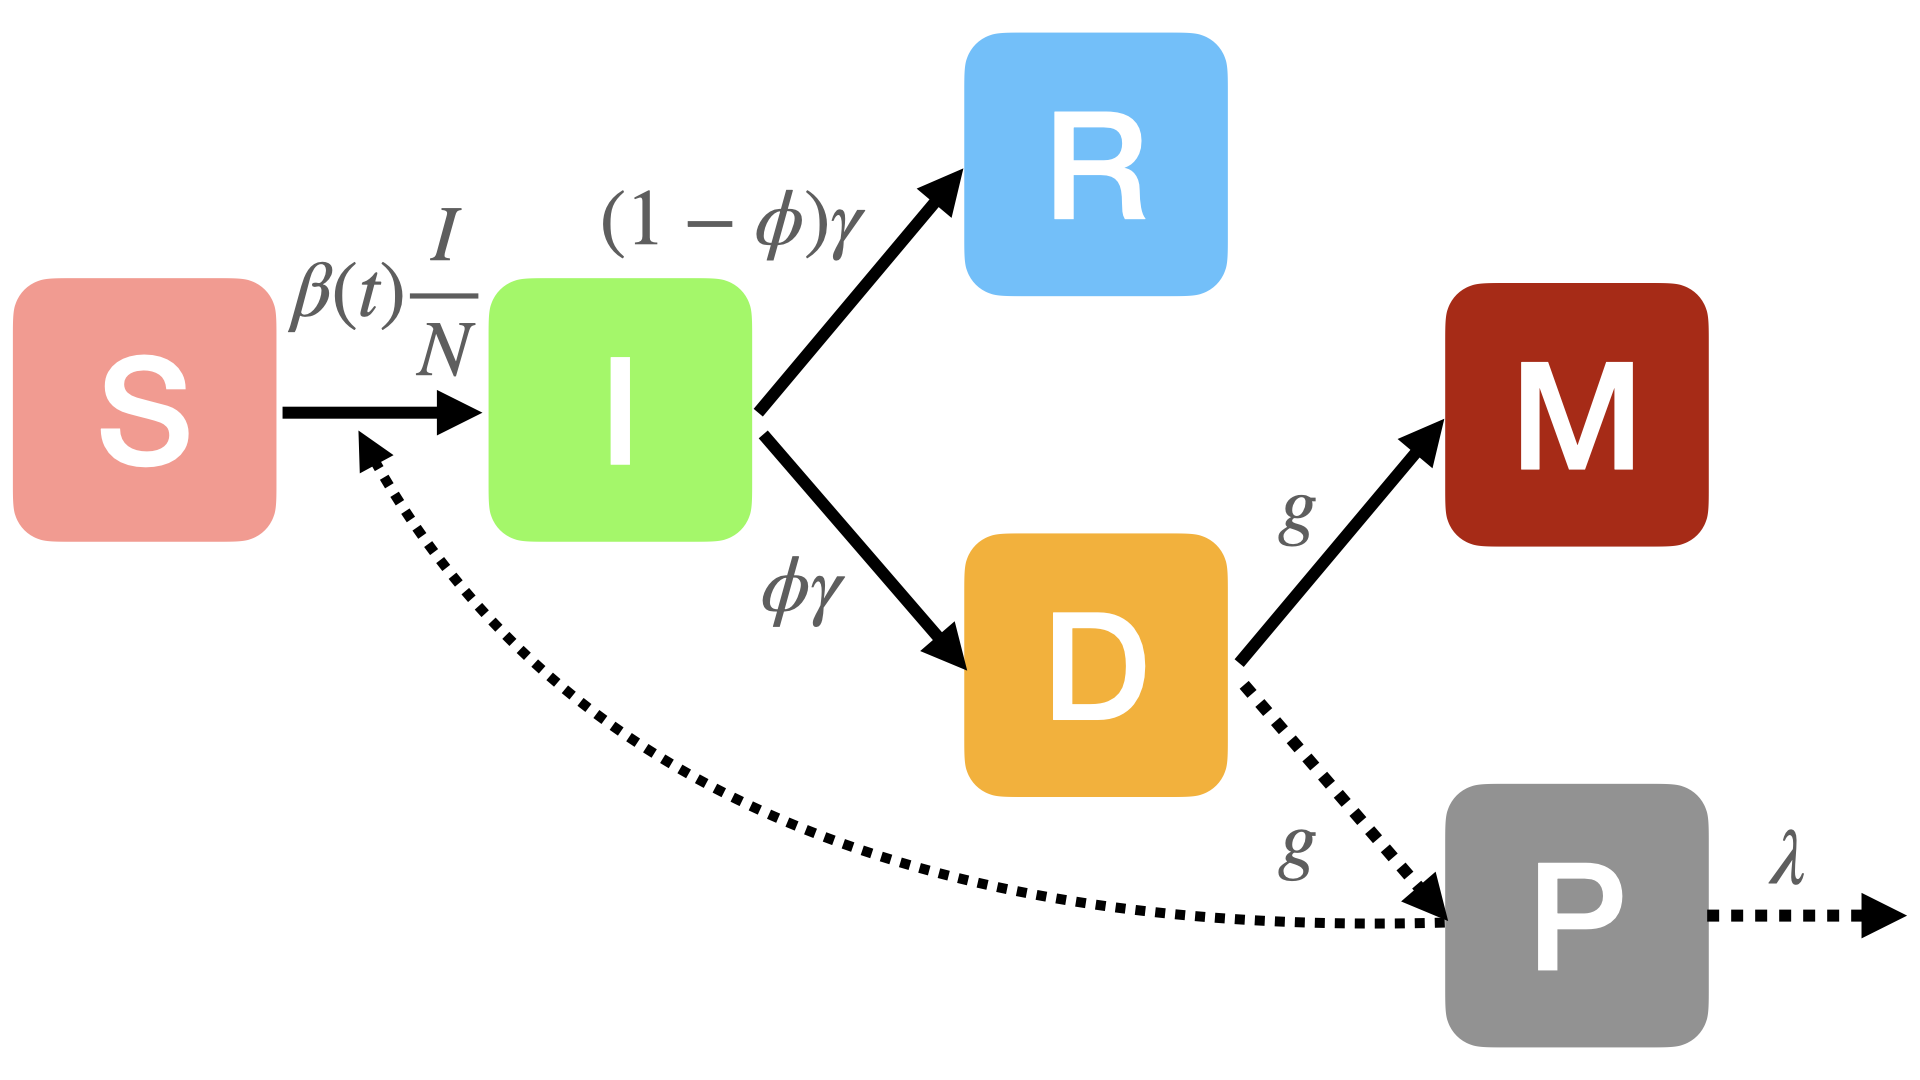
\includegraphics[height=4cm]{../graphics/sir-metapop.png}
\end{center}

\framebreak

\begin{equation*}
\begin{aligned}
  \deriv{S}{t} &= - \beta(t)\,S\,\frac{I}{N}\\
  \deriv{I}{t} &= \beta(t)\,S\,\frac{I}{N} - \gamma\,I \\
  \deriv{R}{t} &= (1-\phi)\,\gamma\,I \\
  \deriv{D}{t} &= \phi\,\gamma\,I \\
  \deriv{M}{t} &= g\,D \\
  \deriv{P}{t} &= g\,D - \lambda\,P
\end{aligned}
\end{equation*}

\begin{itemize}
\tightlist
\item
  \(S\), \(I\), \(R\): the susceptible, infectious, and recovered
  populations
\item
  \(D\): those who have lost of infectiousness and are progressing to
  death due to influenza or/and pneumonia
\item
  \(M\): those who have died
\item
  \(P\): general public's risk perception based on recent influenza
  deaths
\item
  \(N\): \(N=S+I+R+D+M\), the constant total population size
\end{itemize}

\framebreak

The time-dependent transmission rate \(\beta(t)\) consists of two
components:

\begin{equation}
\beta(t) =\beta_{0}\cdot \left(1-\frac{P(t)}{N}\right)^{\kappa}
\end{equation}

\begin{itemize}
\tightlist
\item
  \(\beta_{0}\): the baseline transmission rate
\item
  \(\left(1-\frac{P(t)}{N}\right)^{\kappa}\): represent the effect of
  reactive social distancing on transmission rate based on the public's
  risk perception \(P(t)\)
\end{itemize}

\vfill

The number of reported cases \(C\) follows a Negative Binomial
distribution, in London, Birmingham, and Liverpool, respectively, with
ratio \(\rho\) and over-dispersion parameter \(k\), given the cumulative
number of cases \(H\):

\[
  C \sim \mathrm{NegBin}(\rho H,k)
\]

\framebreak

\begin{itemize}
\tightlist
\item
  Fixed parameters:

  \begin{itemize}
  \tightlist
  \item
    The total population sizes for London, Birmingham, and Liverpool are
    fixed at 4484523, 919444, and 802940, respectively
  \item
    \(\gamma^{-1}\): the average infectious period, fixed at 4 days
  \item
    \(g^{-1}\): the mean time from loss-of-infectiousness to death,
    fixed at 8 days
  \end{itemize}
\item
  Parameters to be estimated, initial conditions:

  \begin{itemize}
  \tightlist
  \item
    \(\eta_L, \eta_B,\eta_L\): the initial fraction of susceptible
    individuals for London, Birmingham, and Liverpool, respectively
  \item
    \(\psi_L,\psi_B,\psi_L\): the initial fraction of infectious
    individuals for London, Birmingham, and Liverpool, respectively
  \end{itemize}
\item
  Parameters to be estimated, common features:

  \begin{itemize}
  \tightlist
  \item
    \(\beta_{0}\): the baseline transmission rate
  \item
    \(\kappa\): the exponent of the social distancing effect
  \item
    \(\lambda\): the rate at which the public's risk perception decays
  \end{itemize}
\end{itemize}

\hypertarget{pomp-setting}{%
\section{POMP setting}\label{pomp-setting}}

\hypertarget{the-implementation-in-pomp-the-state-process-for-meta-populations}{%
\subsection{\texorpdfstring{The implementation in \texttt{pomp}: the
state process for
meta-populations}{The implementation in pomp: the state process for meta-populations}}\label{the-implementation-in-pomp-the-state-process-for-meta-populations}}

\begin{Shaded}
\begin{Highlighting}[]
\NormalTok{sir\_meta }\OtherTok{\textless{}{-}} \FunctionTok{Csnippet}\NormalTok{(}\StringTok{"}
\StringTok{  double *S = \&S1, *I = \&I1, *R = \&R1, *D = \&D1, *M = \&M1;}
\StringTok{  double *P = \&P1, *H = \&H1; int N[3] = \{N1, N2, N3\};}
\StringTok{  double Beta, dN\_SI, dN\_IRD, dN\_IR, dN\_ID, dN\_DM, dN\_P;}
\StringTok{  for (int i = 0; i \textless{} 3; i++) \{}
\StringTok{    Beta = beta0*pow(1{-}P[i]/N[i],kappa);}
\StringTok{    dN\_SI = rbinom(S[i],1{-}exp({-}Beta*I[i]/N[i]*dt));}
\StringTok{    dN\_IRD = rbinom(I[i],1{-}exp({-}gamma*dt));}
\StringTok{    dN\_IR = nearbyint((1{-}phi)*dN\_IRD); dN\_ID = nearbyint(phi*dN\_IRD);}
\StringTok{    dN\_DM = rbinom(D[i],1{-}exp({-}g*dt));}
\StringTok{    dN\_P = rbinom(P[i],1{-}exp({-}lambda*dt));}
\StringTok{    S[i] {-}= dN\_SI; I[i] += dN\_SI {-} dN\_IRD; R[i] += dN\_IR; }
\StringTok{    D[i] += dN\_ID {-} dN\_DM; M[i] += dN\_DM; P[i] += dN\_DM {-} dN\_P;}
\StringTok{    H[i] += dN\_IRD;\}}
\StringTok{"}\NormalTok{)}
\end{Highlighting}
\end{Shaded}

\hypertarget{the-implementation-in-pomp-the-initial-conditions}{%
\subsection{\texorpdfstring{The implementation in \texttt{pomp}: the
initial
conditions}{The implementation in pomp: the initial conditions}}\label{the-implementation-in-pomp-the-initial-conditions}}

\begin{Shaded}
\begin{Highlighting}[]
\NormalTok{sir\_meta\_rinit }\OtherTok{\textless{}{-}} \FunctionTok{Csnippet}\NormalTok{(}\StringTok{"}
\StringTok{  double *S = \&S1, *I = \&I1, *R = \&R1, *D = \&D1, *M = \&M1;}
\StringTok{  double *P = \&P1, *H = \&H1; int N[3] = \{N1, N2, N3\};}
\StringTok{  double eta[3] = \{eta1, eta2, eta3\};}
\StringTok{  double psi[3] = \{psi1, psi2, psi3\};}
\StringTok{  for (int i = 0; i \textless{} 3; i++) \{}
\StringTok{    S[i] = nearbyint(N[i]*eta[i]); }
\StringTok{    I[i] = nearbyint(N[i]*psi[i]); }
\StringTok{    R[i] = nearbyint(N[i]*(1{-}eta[i]{-}psi[i]));}
\StringTok{    D[i] = M[i] = P[i] = H[i] = 0;}
\StringTok{  \}}
\StringTok{"}\NormalTok{)}
\end{Highlighting}
\end{Shaded}

\hypertarget{the-implementation-in-pomp-the-measurements}{%
\subsection{\texorpdfstring{The implementation in \texttt{pomp}: the
measurements}{The implementation in pomp: the measurements}}\label{the-implementation-in-pomp-the-measurements}}

\begin{Shaded}
\begin{Highlighting}[]
\NormalTok{sir\_meta\_dmeas }\OtherTok{\textless{}{-}} \FunctionTok{Csnippet}\NormalTok{(}\StringTok{"}
\StringTok{  double lik1, lik2, lik3;}
\StringTok{  lik1 = (ISNA(London)) ? dnbinom\_mu(London,rho*H1,k,1) : 0;}
\StringTok{  lik2 = (ISNA(Birmingham)) ? dnbinom\_mu(Birmingham,rho*H2,k,1) : 0;}
\StringTok{  lik3 = (ISNA(Liverpool)) ? dnbinom\_mu(Liverpool,rho*H3,k,1) : 0;}
\StringTok{  lik = lik1 + lik2 + lik3;}
\StringTok{  lik = (give\_log) ? lik : exp(lik);}
\StringTok{"}\NormalTok{)}

\NormalTok{sir\_meta\_rmeas }\OtherTok{\textless{}{-}} \FunctionTok{Csnippet}\NormalTok{(}\StringTok{"}
\StringTok{  London = rnbinom\_mu(k,rho*H1);}
\StringTok{  Birmingham = rnbinom\_mu(k,rho*H2);}
\StringTok{  Liverpool = rnbinom\_mu(k,rho*H3);}
\StringTok{"}\NormalTok{)}
\end{Highlighting}
\end{Shaded}

\hypertarget{the-implementation-in-pomp-build-the-model}{%
\subsection{\texorpdfstring{The implementation in \texttt{pomp}: build
the
model}{The implementation in pomp: build the model}}\label{the-implementation-in-pomp-build-the-model}}

\begin{Shaded}
\begin{Highlighting}[]
\NormalTok{dat }\SpecialCharTok{|\textgreater{}} \FunctionTok{select}\NormalTok{(}\SpecialCharTok{{-}}\NormalTok{date) }\SpecialCharTok{|\textgreater{}}
  \FunctionTok{pomp}\NormalTok{(}
    \AttributeTok{times =} \StringTok{"week"}\NormalTok{, }\AttributeTok{t0 =} \DecValTok{0}\NormalTok{, }
    \AttributeTok{rprocess=}\FunctionTok{euler}\NormalTok{(sir\_meta,}\AttributeTok{delta.t=}\DecValTok{1}\SpecialCharTok{/}\DecValTok{7}\NormalTok{),}
    \AttributeTok{rinit=}\NormalTok{sir\_meta\_rinit, }\AttributeTok{rmeasure=}\NormalTok{sir\_meta\_rmeas,}
    \AttributeTok{dmeasure=}\NormalTok{sir\_meta\_dmeas, }\AttributeTok{accumvars =} \FunctionTok{sprintf}\NormalTok{(}\StringTok{"H\%d"}\NormalTok{,}\DecValTok{1}\SpecialCharTok{:}\DecValTok{3}\NormalTok{),}
    \AttributeTok{statenames=}\FunctionTok{c}\NormalTok{(}\FunctionTok{sprintf}\NormalTok{(}\StringTok{"S\%d"}\NormalTok{,}\DecValTok{1}\SpecialCharTok{:}\DecValTok{3}\NormalTok{),}\FunctionTok{sprintf}\NormalTok{(}\StringTok{"I\%d"}\NormalTok{,}\DecValTok{1}\SpecialCharTok{:}\DecValTok{3}\NormalTok{),}
      \FunctionTok{sprintf}\NormalTok{(}\StringTok{"R\%d"}\NormalTok{,}\DecValTok{1}\SpecialCharTok{:}\DecValTok{3}\NormalTok{), }\FunctionTok{sprintf}\NormalTok{(}\StringTok{"D\%d"}\NormalTok{,}\DecValTok{1}\SpecialCharTok{:}\DecValTok{3}\NormalTok{),}\FunctionTok{sprintf}\NormalTok{(}\StringTok{"M\%d"}\NormalTok{,}\DecValTok{1}\SpecialCharTok{:}\DecValTok{3}\NormalTok{),}
      \FunctionTok{sprintf}\NormalTok{(}\StringTok{"P\%d"}\NormalTok{,}\DecValTok{1}\SpecialCharTok{:}\DecValTok{3}\NormalTok{),}\FunctionTok{sprintf}\NormalTok{(}\StringTok{"H\%d"}\NormalTok{,}\DecValTok{1}\SpecialCharTok{:}\DecValTok{3}\NormalTok{)),}
    \AttributeTok{paramnames=}\FunctionTok{c}\NormalTok{(}
      \StringTok{"beta0"}\NormalTok{,}\StringTok{"kappa"}\NormalTok{,}\StringTok{"gamma"}\NormalTok{,}\StringTok{"phi"}\NormalTok{,}\StringTok{"g"}\NormalTok{,}\StringTok{"lambda"}\NormalTok{,}\StringTok{"rho"}\NormalTok{,}\StringTok{"k"}\NormalTok{, }
      \FunctionTok{sprintf}\NormalTok{(}\StringTok{"N\%d"}\NormalTok{,}\DecValTok{1}\SpecialCharTok{:}\DecValTok{3}\NormalTok{),}\FunctionTok{sprintf}\NormalTok{(}\StringTok{"eta\%d"}\NormalTok{,}\DecValTok{1}\SpecialCharTok{:}\DecValTok{3}\NormalTok{),}\FunctionTok{sprintf}\NormalTok{(}\StringTok{"psi\%d"}\NormalTok{,}\DecValTok{1}\SpecialCharTok{:}\DecValTok{3}\NormalTok{))}
\NormalTok{  ) }\OtherTok{{-}\textgreater{}}\NormalTok{ pomp\_meta}
\end{Highlighting}
\end{Shaded}

\framebreak

\begin{Shaded}
\begin{Highlighting}[]
\NormalTok{params }\OtherTok{\textless{}{-}} \FunctionTok{c}\NormalTok{(}\AttributeTok{beta0 =} \DecValTok{5}\NormalTok{, }\AttributeTok{kappa =} \DecValTok{5}\NormalTok{, }\AttributeTok{gamma =} \DecValTok{1}\SpecialCharTok{/}\DecValTok{4}\NormalTok{, }\AttributeTok{phi =} \FloatTok{0.0119}\NormalTok{, }\AttributeTok{g =} \DecValTok{1}\SpecialCharTok{/}\DecValTok{8}\NormalTok{, }
  \AttributeTok{lambda =} \DecValTok{1}\SpecialCharTok{/}\DecValTok{2}\NormalTok{, }\AttributeTok{rho =} \FloatTok{0.05}\NormalTok{, }\AttributeTok{k =} \DecValTok{10}\NormalTok{, }\AttributeTok{N1 =} \DecValTok{4484523}\NormalTok{, }\AttributeTok{N2 =} \DecValTok{919444}\NormalTok{, }
  \AttributeTok{N3 =} \DecValTok{802940}\NormalTok{, }\AttributeTok{eta1 =} \FloatTok{0.2}\NormalTok{, }\AttributeTok{eta2 =} \FloatTok{0.2}\NormalTok{, }\AttributeTok{eta3 =} \FloatTok{0.2}\NormalTok{, }
  \AttributeTok{psi1 =} \FloatTok{0.0005}\NormalTok{, }\AttributeTok{psi2 =} \FloatTok{0.0005}\NormalTok{, }\AttributeTok{psi3 =} \FloatTok{0.0005}\NormalTok{)}

\NormalTok{pomp\_meta }\SpecialCharTok{|\textgreater{}} 
  \FunctionTok{simulate}\NormalTok{(}
    \AttributeTok{params =}\NormalTok{ params, }\AttributeTok{nsim=}\DecValTok{20}\NormalTok{,}\AttributeTok{format=}\StringTok{"data.frame"}\NormalTok{,}\AttributeTok{include.data=}\ConstantTok{TRUE}
\NormalTok{  ) }\SpecialCharTok{|\textgreater{}}
  \FunctionTok{select}\NormalTok{(week,.id,London,Birmingham,Liverpool) }\SpecialCharTok{|\textgreater{}}
\NormalTok{  reshape2}\SpecialCharTok{::}\FunctionTok{melt}\NormalTok{(}\AttributeTok{id.vars =} \FunctionTok{c}\NormalTok{(}\StringTok{"week"}\NormalTok{,}\StringTok{".id"}\NormalTok{)) }\SpecialCharTok{|\textgreater{}}
  \FunctionTok{ggplot}\NormalTok{(}\FunctionTok{aes}\NormalTok{(}\AttributeTok{x=}\NormalTok{week, }\AttributeTok{y=}\NormalTok{value, }\AttributeTok{group=}\NormalTok{.id, }\AttributeTok{color=}\NormalTok{.id}\SpecialCharTok{==}\StringTok{"data"}\NormalTok{)) }\SpecialCharTok{+}
  \FunctionTok{geom\_line}\NormalTok{() }\SpecialCharTok{+} \FunctionTok{facet\_wrap}\NormalTok{(variable }\SpecialCharTok{\textasciitilde{}}\NormalTok{ .) }\SpecialCharTok{+} 
  \FunctionTok{theme\_minimal}\NormalTok{() }\SpecialCharTok{+} \FunctionTok{guides}\NormalTok{(}\AttributeTok{color=}\StringTok{"none"}\NormalTok{)}
\end{Highlighting}
\end{Shaded}

\framebreak

\begin{figure}[h!]

{\centering 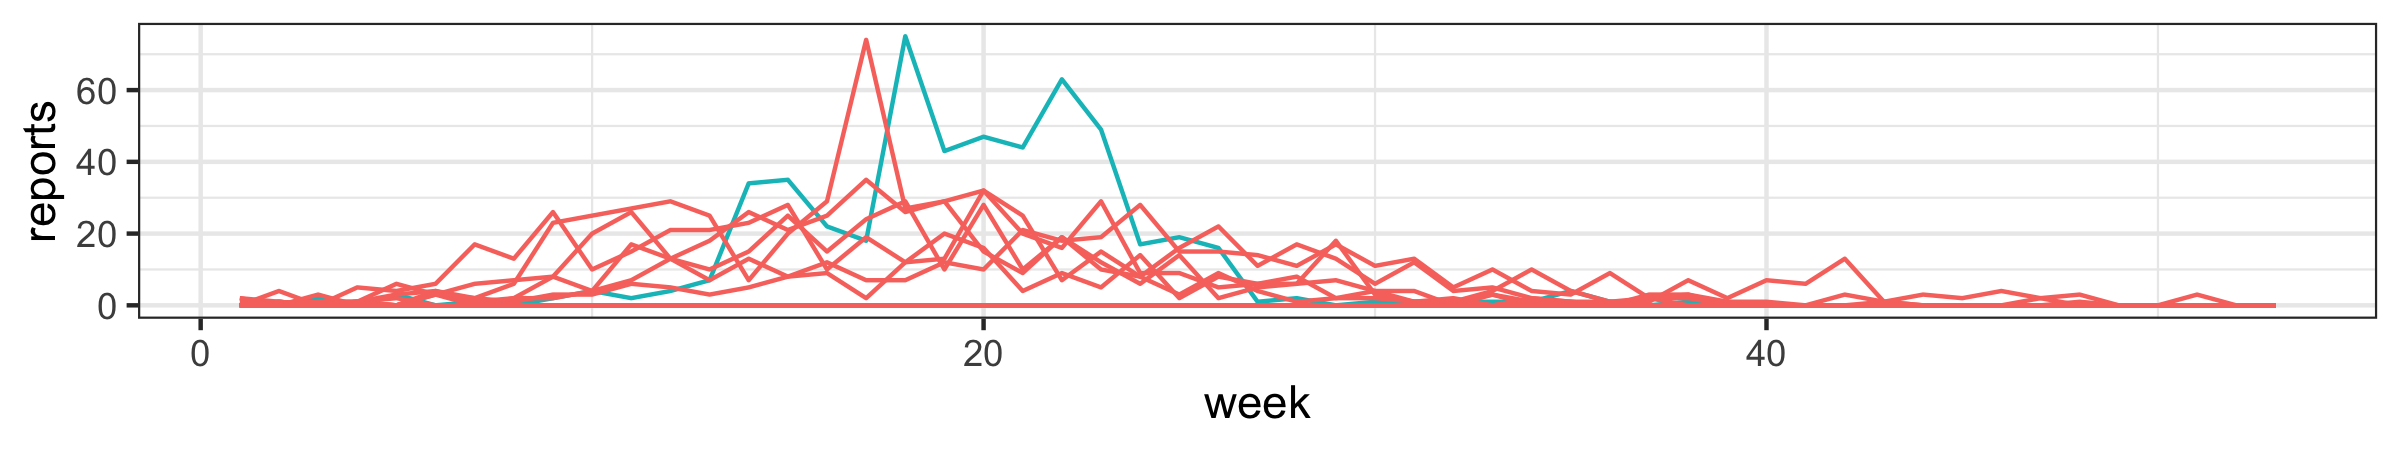
\includegraphics[width=\textwidth,height=0.9\textheight]{tmp//figure/unnamed-chunk-1-1.png}

}

\end{figure}

\hypertarget{license-acknowledgments-and-links}{%
\subsection{License, acknowledgments, and
links}\label{license-acknowledgments-and-links}}

\begin{itemize}
\item
  This lesson is prepared for the
  \href{https://rubbislam.quarto.pub/episim/}{Simulation-based Inference
  for Epidemiological Dynamics} module at the Summer Institute in
  Statistics and Modeling in Infectious Diseases,
  \href{https://sph.emory.edu/SISMID/index.html}{SISMID}.
\item
  The materials build on \href{../acknowledge.html}{previous versions of
  this course and related courses}.
\item
  Licensed under the
  \href{https://creativecommons.org/licenses/by-nc/4.0/}{Creative
  Commons Attribution-NonCommercial license}. Please share and remix
  non-commercially, mentioning its origin.
  
\includegraphics[height=12pt]{../graphics/cc-by-nc}
\item
  Produced with R version 4.3.2 and pomp version 5.10.
\item
  Compiled on 2024-07-24.
\end{itemize}

\vfill

\href{index.html}{Back to Lesson}

\href{./main.R}{\texttt{R} code for this lesson}



\end{document}
